%  !TeX  root  =  sigll.tex
\chapter{Exercices}

\section{Importer des données}

\subsection{Importer des vecteurs}

Ouvrez le menu \mainmenuopt{Couches} \arrow \dropmenuopttwo{mActionAddOgrLayer.png}{Ajouter une couche vecteur}

Cliquez sur le bouton \button{Parcourir} et sélectionnez dans la liste déroulante le format \textbf{ESRI Shapefile}

Sélectionnez dans le dossier ressources/vecteurs les fichiers \filename{eau.shp} et \filename{jardin.shp}

Cliquez sur \button{Ouvrir} pour finaliser l'opération.

Répétez la manipulation en sélectionnant cette fois \textbf{Mapinfo} comme format et le fichier \filename{bati mapinfo.mif}

\subsection{Importer des rasters}

Ouvrez le menu \mainmenuopt{Couches}\arrow\dropmenuopttwo{mActionAddRasterLayer.png}{Ajouter une couche raster}, 

Sélectionnez le format \textbf{GeoTIFF} puis les fichiers \filename{srtm bassin parisien.tif} et \filename{srtm ombrage.tif} 

Cliquez sur \button{Ouvrir}.

\section{Bases de l'interface}

\begin{figure}[ht]
   \centering
   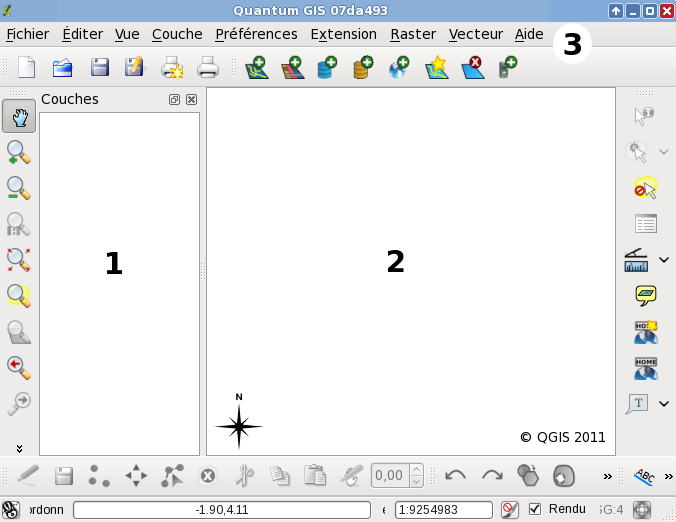
\includegraphics[clip=true, width=10cm]{interface}
\end{figure}

\begin{itemize}
\item 1 - légende cartographie : liste les couches chargées dans le projet
\item 2 - canevas : affiche les couches actives
\item 3 - menus : permet l'accès aux fonctions
\end{itemize}

\subsection{Agencer les couches}

Faites un clic droit sur la zone de légende puis choisissez \dropmenuopt{Ajouter un groupe}. Un nouveau dossier apparaît où vous pouvez maintenant glisser et déposer les couches sur l'icône de ce dossier. 

Créez un groupe Vecteurs et un groupe Rasters. Pour changer le nom du groupe, sélectionnez \dropmenuopt{Renommer} dans le menu contextuel du groupe.

\subsection{Centrer l'affichage}

Décochez la case du groupe Rasters afin de ne plus afficher les couches qu'il contient.

Sélectionnez le groupe Vecteurs, faites un clic-droit et cliquez sur \dropmenuopt{Zoomer sur le groupe}.

\section{Préférences}\label{sec:} 

\subsection{Propriétés du projet}

Ouvrez le menu \mainmenuopt{Préférences}\arrow \dropmenuopttwo{mActionProjectProperties.png}{Propriétés du projet}, déplacez-vous dans l'onglet \dialog{Système de coordonnées de référence}. Cet onglet permet d'indiquer à QGIS le système général à utiliser pour le projet.

Dans la case Rechercher, tapez l'identifiant LAMB1 puis le bouton \button{Trouver}. La liste présente dans la partie supérieure se focalise sur le système correspondant à ce code, à savoir la projection Lambert 1 telle qu'exprimée dans le registre IGNF.

Cochez la case \checkbox{Activer la projection 'à la volée'}, elle permet de reprojeter des couches vectorielles ou raster vers le système général sans devoir les exporter vers celui-ci.

\subsection{Options générales}

Ouvrez le menu \mainmenuopt{Préférences}\arrow \dropmenuopttwo{mActionOptions}{Options}.

Déplacez-vous dans l'onglet \tab{Outils cartographiques} et \selectstring{ellipsoïde pour les mesures de distances}{GRS 1980}.


\section{Utiliser l'interface}\label{sec:ui_use} 

\subsection{Sélectionner des entités}

Sélectionnez la couche \filename{jardin}.

Dans la barre d'outils \textit{Attributs}, cliquez sur l'outil \dropmenuopttwo{mActionSelect}{Sélection d'entités}.

Cliquez sur un objet du canevas, utilisez la touche \keystroke{Ctrl} pour faire une sélection multiple.

Cliquez sur \dropmenuopttwo{mActionDeselectAll}{Désélectionner toutes les entités}.

\subsection{Identification}

Cliquez sur le bouton \dropmenuopttwo{mActionIdentify}{Identifier les entités} puis sur une entité.

Obtenez la surface en dépliant la ligne \textit{(Dérivé)}.

\subsection{Mesurer une longueur, une aire et un angle}

Pour sélectionner un outil de mesure, cliquez sur 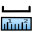
\includegraphics[width=0.7cm]{mActionMeasure} puis sur l'outil voulu.

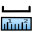
\includegraphics[width=0.7cm]{mActionMeasure} 
\qg peut mesurer des distances réelles entre plusieurs points selon un ellipsoïde défini. \par
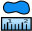
\includegraphics[width=0.7cm]{mActionMeasureArea} Les aires peuvent aussi être mesurées.
Dans la fenêtre de mesure apparaît la surface totale mesurée. \par
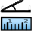
\includegraphics[width=0.7cm]{mActionMeasureAngle}
Le curseur adopte une forme en croix. Cliquez pour dessiner le premier côté de l'angle à mesurer puis bouger le curseur pour dessiner l'angle désiré.

\subsection{Signets spatiaux} \label{sec:bookmarks}

Les signets spatiaux vous permettent de marquer une zone de la carte pour y retourner plus tard.

\minisec{Créer un signet}
Pour créer un signet :
\begin{enumerate}
\item Déplacez-vous sur une zone précise
\item Sélectionnez le menu \mainmenuopt{Vue} > \dropmenuopt{Nouveau signet} ou appuyez sur le bouton \dropmenuopttwo{mActionNewBookmark}{Nouveau signet...}
\item Entrez un nom pour décrire le signet (jusqu'à 255 caractères)
\item Cliquez sur \button{OK} pour ajouter le signet ou sur \button{Annuler} pour sortir de la fenêtre sans l'enregistrer
\end{enumerate}

\minisec{Zoomer sur un signet}
Cliquez sur le bouton \dropmenuopttwo{mActionShowBookmarks}{Montrer les signets}, sélectionnez le signet voulu en cliquant dessus puis sur le bouton \button{Zoomer sur}. Vous pouvez aussi zoomer en opérant un double-clic.

\subsection{Outils d'annotation}

Cliquez sur 
\includegraphics[width=0.7cm, clip=true]{mActionTextAnnotation} dans la barre d'outils d'attribut puis cliquez sur le canevas.

Faites un double-clic sur l'annotation pour éditer le texte.

\subsection{La table attributaire}

Cliquez sur le bouton 
\includegraphics[width=0.7cm]{mActionOpenTable} qui permet d'ouvrir la table attributaire ou par un clic droit sur la couche \filename{jardin}. 

\minisec{Sélectionner une entité depuis la table}
Pour une simple recherche par attribut sur une seule colonne, le champ \button{Chercher pour} peut être utilisé. Sélectionnez la colonne \textit{NOM} sur laquelle doit être opérée la recherche depuis la liste déroulante, tapez \textit{Binet} et appuyez sur le bouton \button{Chercher}. 

Cliquez sur le bouton \toolbtntwo{mActionZoomToSelected}{Zoomer la carte sur les lignes sélectionnées}

\section{Symbologie}

Pour accéder à la fenêtre \dialog{Propriétés de la couche}, double-cliquez sur la couche \textit{jardin} dans la légende ou faites un clic droit sur la couche et sélectionnez \dropmenuopt{Propriétés} dans le menu qui apparait.

L'onglet \textbf{Style} est affiché, la représentation par défaut est le symbole unique où un style unique est appliqué à tous les objets de la couche. On peut d'ici modifier la \textbf{couleur} et la \textbf{transparence} de la couche.
        
\section{Symbologie avancée}

\subsection{Classifier}

Pour opérer une classification des éléments de la couche, il faut passer dans la liste de \textit{symbole unique} à \textit{catégorisé} et choisir la colonne qui permettra de définir les différentes classes, ici la colonne \textit{DENOM}. Cliquez ensuite sur le bouton \button{Classer}, QGIS créé une liste des classes en déclinant une palette de couleurs.

Plutôt que de changer les couleurs manuellement nous allons charger le style \filename{style jardin classification.qml} depuis le bouton \button{Charger le style}.

\subsection{Étiqueter}

Allez dans le menu \mainmenuopt{Couches}\arrow\dropmenuopttwo{labeling}{Étiquetage}.

Sélectionner \selectstring{Champ contenant les étiquettes}{NOM} et cochez la case \checkbox{Étiqueter cette couche}.

\section{Composer une carte}

Cliquez sur l'icône 
\includegraphics[width=0.7cm]{mActionNewComposer} ou le menu \mainmenuopt{Fichier} > \dropmenuopttwo{mActionNewComposer}{Nouveau composeur d'impression}.

Le composeur de carte affiche deux onglets :

\begin{itemize}[label=--]
\item L'onglet \tab{Général} vous permet de définir la taille du papier, l'orientation et la qualité d'impression pour le fichier de sortie (en dpi/ppp) et d'activer l'accrochage sur une grille d'une résolution prédéfinie.
\item L'onglet \tab{Objet} affiche les propriétés pour l'élément de la carte sélectionnée. Cliquez sur l'icône \toolbtntwo{mActionSelectPan}{Sélectionner/Déplacer l'objet}  pour sélectionner un élément (par exemple l'échelle graphique ou une étiquette) dans le cadre. Puis cliquez sur l'onglet Item et personnalisez les paramètres pour l'élément sélectionné.
\item L'onglet \tab{Historique des commandes} permet de d'annuler ou refaire des manipulations.
\end{itemize}

Ajoutez une vue sur le canevas de la carte en utilisant le bouton 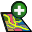
\includegraphics[width=0.7cm]{mActionAddMap}.

Déplacez le contenu de la vue en utilisant le bouton 
\includegraphics[width=0.7cm]{mActionSelectPan}.

Ajoutez une échelle graphique en utilisant le bouton 
\includegraphics[width=0.7cm]{mActionScaleBar} et en cliquant sur la feuille.

Ajoutez une flèche pointant vers le Nord en utilisant le bouton 
\includegraphics[width=0.7cm]{mActionSaveMapAsImage} et en cliquant sur la carte puis sélectionnez le cadre et déplacez-vous dans l'onglet \textit{Objet}. Dans le cadre d'aperçu, sélectionnez une image de flèche.

Exporter le résultat en PDF en appuyant sur le bouton 
\includegraphics[width=0.7cm]{mActionSaveAsPDF}.